\chapter{Deep Deterministic Policy Gradient (DDPG)}
As we stated in the last chapter, we have chosen the DDPG algorithm based on the nature of our problem so we now introduce the algorithm as the basic idea then we will go deeper to formulate our problem in the algorithm later this chapter.\\
To fully understand DDPG we must first walk through Actor-Critic algorithms family.

\section{ACTOR-CRITIC Methods}
\begin{wrapfigure}{h}{0.55\textwidth}
    \centering
    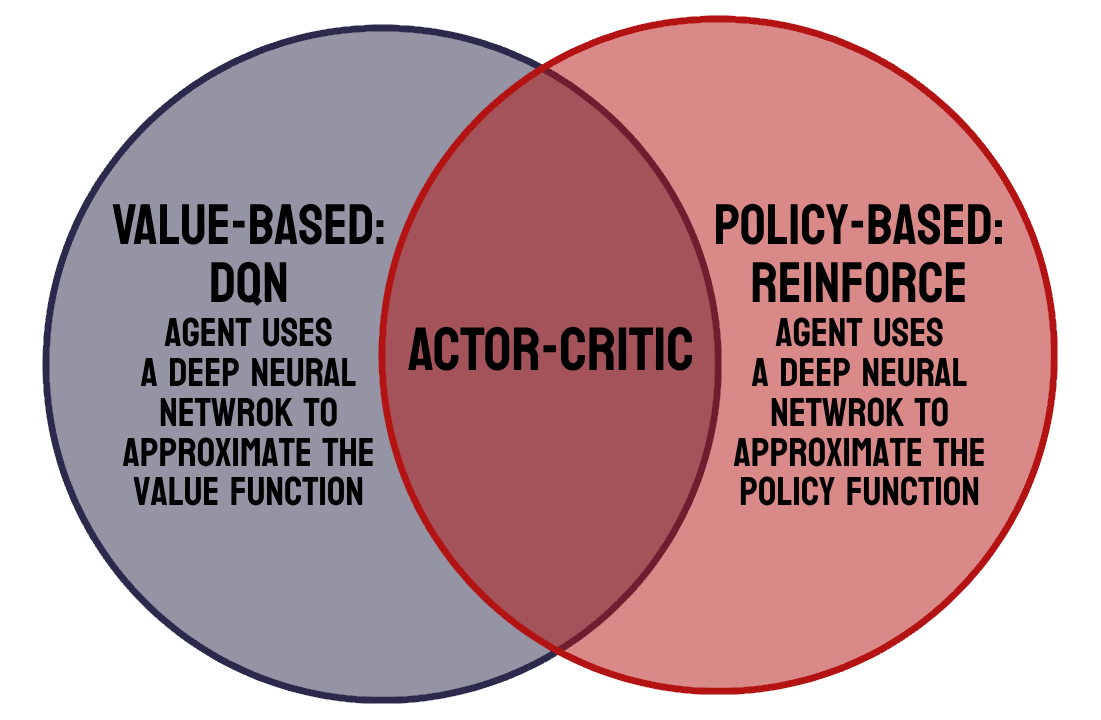
\includegraphics[width=0.55\textwidth]{41.PNG}
    \caption{ACTOR-CRITIC Methods}
    \label{fig:ACTOR-CRITIC Methods}
\end{wrapfigure}

Figure~\ref{fig:ACTOR-CRITIC Methods} depicts the main concept of Actor-Critic methods. Actor-Critic methods combine the \textbf{value-based methods} such as DQN and \textbf{policy-based methods} such as Reinforce.\\
DQN Agent which learns to approximate the optimal action value function. If the Agent learns sufficiently well so deriving a good policy for the Agent, it is straightforward.
On the other side the Reinforce Agent parametrizes the policy and learns to optimize it directly. Here, the policy is usually stochastic, as we receive the distribution probability.\\
Right now, we will investigate deterministic policies, which take a state and return the single action (no stochasticity, the policy will be deterministic).\\
\begin{description}
    \item[For Reinforce Algorithm:] it has to complete the episode before we can start training. For the environments, where every episode can last hundreds or even thousands of frames (like Atari games). It can be wasteful for the training perspective, where we have to interact with the environment in long perspective, only just to perform a single training step (in order to estimate $\mathbf{Q}$ as accurate as possible). In this case, the training batch becomes very large.
    \item[For DQN:] it is possible to replace the exact value for a discounted reward with our estimation using the one-step Bellman equation:
    \[ \mathbf{Q}(s,a) = r + \gamma \mathbf{V}( \mathbf{S}' ) \]
    When we consider the Policy Gradient method (as we discussed above), we contemplated that the values $\mathbf{V}(\mathbf{S})$ or $\mathbf{Q}\left(s,a\right)$ exist anymore. In this case we apply the Actor-Critic method instead, where we use neural network to estimate $\mathbf{V}(\mathbf{S})$ and use this estimation to obtain $\mathbf{Q}$.
\end{description}

\begin{wrapfigure}{h}{0.5\textwidth}
    \centering
    \vspace{-20pt}
    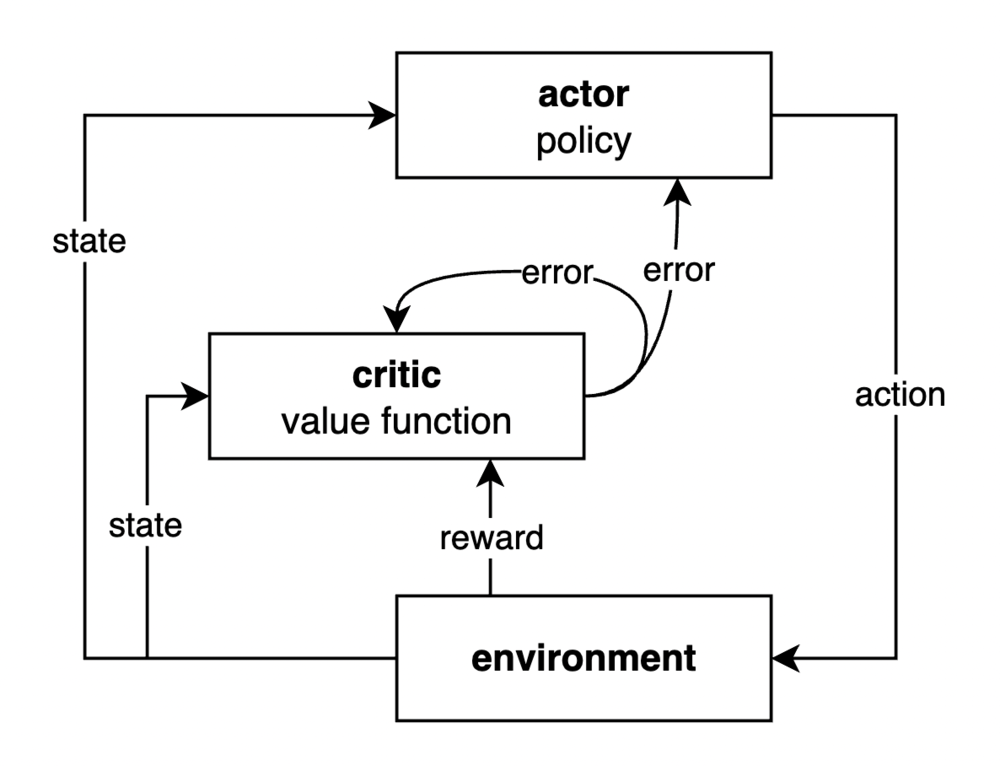
\includegraphics[width=0.5\textwidth]{42.PNG}
    \caption{ACTOR-CRITIC}
    \label{fig:ACTOR-CRITIC algo}
\end{wrapfigure}

Estimated gradient in Policy Gradient method is proportional to the discounted reward from the given state. However, the range of this reward is highly environment dependent (it can happen that the Agent plays only short game the Agent lose very quick (low value of reward) or the Agent is smart enough and plays the game for the longer time, while collecting the rewards). Large difference between rewards collection can seriously affect the training dynamics, as one lucky episode will dominate in the final gradient. In such occurrences, the policy gradient method has high variance, which can influence the training process can become unstable.

\section{DDPG Algorithm}
\begin{wrapfigure}{h}{0.5\textwidth}
    \centering
    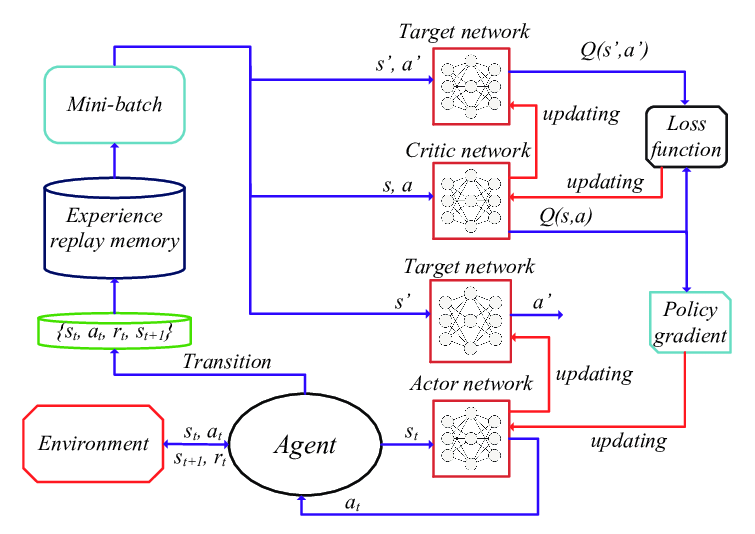
\includegraphics[width=0.5\textwidth]{43.PNG}
    \caption{DDPG Algorithm}
    \label{fig:DDPG algo}
\end{wrapfigure}

In Dynamic Programming, the Markov Decision Process (MDP) is solved by using value iteration and policy iteration. Both techniques require transition and reward probabilities to find the optimal policy. When the transition and reward probabilities are unknown, we use the Monte Carlo method to solve MDP. The Monte Carlo method requires only sample sequences of states, actions, and rewards. Monte Carlo methods are applied only to episodic tasks.\\
We can approach the Monte-Carlo estimate by considering that the Agent play in episode A. We start in state $\mathbf{S}_t$ and act $\mathbf{A}_t$. Based on the process the Agent transits to state $\mathbf{S}_{t+1}$. From environment, the Agent receives the reward $\mathbf{R}_{t+1}$. This process can be continued until the Agent reaches the end of the episode. The Agent can also take part in other episodes like B, C, and D. Some of those episodes will have trajectories that go through the same states, which influences that the value function is computed as average of estimates. Estimates for a state can vary across episodes so the Monte-Carlo estimates will have high variance. \\
On the other side, we can apply the Temporal Difference estimate. Here, the $\mathbf{T}\mathbf{D}$ approximates the current estimate based on the previously learned estimate, which is also called bootstrapping (we try to predict the state values).
\begin{equation}
    \label{eq:Expected reward}
    \begin{aligned}
        \mathbf{V}(\mathbf{S}) = \mathbf{V}(\mathbf{S}) + & \alpha \left( r + \gamma \mathbf{V}(\mathbf{S}') - \mathbf{V}(\mathbf{S}) \right) \\
        \mathbf{V}(\mathbf{S}) & \text{ is the \emph{expected reward}}. \\
        \left( r + \gamma \mathbf{V}(\mathbf{S}') \right) & \text{ is the \emph{actual reward}}.
    \end{aligned}
\end{equation}
Equation~\ref{eq:Expected reward} is the difference ($\mathbf{T}\mathbf{D}$ error) between the actual reward and the expected reward multiplied by the learning rate $\alpha$ (the learning rate, also called step size, used for convergence reason).
$\mathbf{T}\mathbf{D}$ estimates are low variance because you are only compounding a single time step of randomness instead of a full rollout like in Monte-Carlo estimate. However, due to applying bootstrapping (dynamic programming) the next state is only estimated. Estimated values introduce bias into our calculations. The agent will learn faster, but converging problems can occur.
Deriving the Actor -Critic concept requires to consider first the policy-based approach \emph{(performed by AGENT)}.\\
As we discussed before, the Agent playing the game increases the probability of actions that lead to a win and decreases the probability of actions that lead to losses. However, such a process is cumbersome due to a lot of data to approach the optimal policy.
On the other hand, we can evaluate the value-based approach \emph{(performed by CRITIC)}, where the guesses are performed on-the-fly, throughout all the episodes. At the beginning our guesses will be misaligned (not correct). But over time, when we capture more experience, we will be able to make solid guesses. Though this is not a perfect approach either, guesses introduce a bias because they will sometimes be wrong, particularly because of a lack of experience.
\begin{GrayBox}
    \textbf{We can summarize that:}
    \begin{itemize}
        \item The Agent using policy-based approach is learning to act (agent learns by interacting with environment and adjusts the probabilities of good and bad actions, while in a value-based approach, the agent is learning to estimate states and actions.).
        \item The Critic is used to evaluate the quality of actions more quickly (proper action or not) and speed up learning.
    \end{itemize}
    As a result of the merger of Actor-Critic we utilize \emph{two separate neural networks}. The role of the Actor network is to determine the best actions (from probability distribution) in the state by tuning the parameter $\theta$ (weights). The Critic, by computing the temporal difference error $\mathbf{T}\mathbf{D}$ (estimating expected returns), evaluates the action generated by the actor.
\end{GrayBox}

(DQN) is working in discrete environments where the number of action which could be performed by the Agent was limited. However, very often we operate with a continuous environment, securing continuous motion. The number of actions then can be unlimited (huge). This is one of the problems DDPG solves. DDPG algorithm uses Agent- Critic concept, where we use two deep neural networks. \\
In DDPG, the Actor is used to approximate the optimal policy deterministically. That means we want always to generate the best believed action for any given state. \\
The Actor follows the policy-based approach and learns how to act by directly estimating the optimal policy and maximizing reward through gradient ascent. The Critic, however, utilizes the value-based approach and learns how to estimate the value of different state-action pairs.

\subsection{Algorithm Steps}
The DDPG algorithm can be presented as follows:
\begin{enumerate}
    \item The Actor and the Critic use \emph{separate} neural networks.
    \item Define the Actor network with
    \begin{equation}
        \label{eq:Actor network}
        a = \mu(s, \theta^\mu)
    \end{equation}
    which takes input as a state $s$ and results in the action $a$ where $\theta^\mu$ is the Actor network learning weights. The actor here is used to approximate the optimal policy deterministically. That means that the output is the best believed action for any given state. This is unlike a stochastic policy (probability distribution) in which we want the policy to learn a probability distribution over the actions. \\
    In DDPG, we want the believed best action every single time we query the actor network. The actor is basically learning the argmax of $\mathbf{Q}\left(s,a\right)$, which is the best action.
    \item Define the Critic network
    \begin{equation}
        \label{eq:Critic network}
        \mathbf{Q}\left( s; a, \theta^Q \right) \Rightarrow \mathbf{Q}\left( s; \mu(s; \theta^\mu), \theta^Q \right)
    \end{equation}
    which takes an input as a state $s$ and action $a$ and returns the $\mathbf{Q}$ value where $\theta^Q$ is the Critic network weights. \\
    The critic learns to evaluate the optimal action value function by using the actors best believed action.
    \item We define a target networks $\mu(s;\theta^{\mu'})$ , $\mathbf{Q}\left( s; a, \theta^{Q'} \right)$ for both the Actor network and Critic network respectively where $\theta^{\mu'}$ , $\theta^{Q'}$ are the weights of the target Actor and Critic network.
    \item Next, we perform the update of Actor network weights with policy gradients and the Critic network weight with the gradients calculated from the $\mathbf{T}\mathbf{D}$ error.
    \item In order, to select correct action, first we have to add an exploration noise $N$ to the action produced by Actor $\mu(s;\theta^{\mu'}) + N$. The noise is added to encourage exploration since the policy is deterministic.
    \item Selected action in a state $s$, receive a reward $r$ and move to a new state $s'$.
    \item We store this transition information in an experience replay buffer.
    \item As it is performed while we use DQN algorithm, we sample transitions from the replay buffer and train the network, and then we calculate the target $\mathbf{Q}$ value
    \begin{equation}
        \label{eq:Target Q value}
        y_i = r_i + \gamma \mathbf{Q}' \left( s_{i+1}, \mu'\left( \theta^{\mu'} | \theta^{Q'} \right) \right)
    \end{equation}
    \item Then, we can compute the $\mathbf{T}\mathbf{D}$ error as
    \begin{equation}
        \label{eq:Loss}
        L = \frac{1}{M} \sum_{i}\left( y_i - \mathbf{Q}\left( s_i, a_i | \theta^Q \right)^2 \right)
    \end{equation}
    \item Subsequently, we perform the update of the Critic networks weights with gradients calculated from this loss $L$.
    \item Update our policy network weights using a policy gradient.
    \item Next, we update the weights of Actor and Critic network in the target network. In DDPG algorithm topology consist of two copies of network weights for each network, (Actor: regular and target) and (Critic: regular and target). In DDPG, the target networks are updated using a soft updates strategy. A soft update strategy consists of slowly blending regular network weights with target network weights. In means that every time step we make our target network be 99.99 percent of target network weights and only a 0.01 percent of regular network weights (slowly mix of regular network weights into target network weights).
    \item We update the weights of the target networks (as show in equation~\ref{eq:update algo weights}) slowly, which promotes greater stability (soft updates strategy).
    \begin{equation}
        \label{eq:update algo weights}
        \begin{aligned}
            \theta^{Q'} & \gets \text{ } \tau \theta^Q + (1- \tau) \theta^{Q'} \\
            \theta^{\mu'} & \gets \text{ } \tau \theta^\mu + (1- \tau) \theta^{\mu'}
        \end{aligned}
    \end{equation}
\end{enumerate}

\subsection{DDPG Algorithm Pseudocode}
The algorithm can be expressed in the form of a pseudocode as shown in Algorithm~\ref{alg:ddpg}.
\begin{algorithm}
    \caption{DDPG Algorithm}
    \label{alg:ddpg}
    \begin{algorithmic}
        \State Randomly initialize critic network $Q(s,a|\theta^Q)$ and actor $\mu(s|\theta^{\mu})$ with weights $\theta^Q$ and $\theta^{\mu}$.
        \State Initialize target network $Q'$ and $\mu'$ with weights $\theta^{Q'} \gets \theta^Q$ and $\theta^{\mu'} \gets \theta^{\mu}$.
        \State Initialize replay buffer $R$.
        \For{episode = 1, M}
            \State Initialize a random process $\mathcal{N}$ for action exploration.
            \State Receive initial observation state $s_1$.
            \For{t=1 , T}
                \State Select action $a_t = \mu\left( s_t | \theta^{\mu} \right) + \mathcal{N}_t$ according to the current policy and exploration noise.
                \State Execute action $a_t$ and observe reward $r_t$ and new state $s_{t+1}$.
                \State Store transition $(s_t, a_t, r_t, s_{t+1})$ in $R$.
                \State Sample a random mini-batch of $N$ transitions $(s_t, a_t, r_t, s_{t+1})$ from $R$.
                \State Set
                \[ y_i = r_i + \gamma \mathbf{Q}' \left( s_{i+1}, \mu'\left( s_{i+1} | \theta^{\mu'} \right) | \theta^{Q'} \right) \]
                \State Update critic by minimizing the loss
                \[ L = \frac{1}{N} \sum_{i}\left( y_i - \mathbf{Q}\left( s_i, a_i | \theta^Q \right)^2 \right) \]
                \State Update the actor policy using the sampled policy gradient
                \[ \nabla_{\theta^\mu} J \approx \frac{1}{N} \sum_{i}\left( \nabla_a Q(s,a|\theta^Q)|_{s=s_i, a= \mu(s_i)} \cdot \nabla_{\theta^{\mu}} \mu \left( s | \theta^{\mu} \right) \right) \]
                \State Update the target networks
                \[ \theta^{Q'} \gets \tau \theta^Q + (1- \tau) \theta^{Q'} \]
                \[ \theta^{\mu'} \gets \tau \theta^\mu + (1- \tau) \theta^{\mu'} \]
            \EndFor
        \EndFor 
    \end{algorithmic}
\end{algorithm}